\subsubsection{Server}
\label{ssub:server}
  Der Nodejs Server stellt die zuvor definierten Endpunkte mittels \texttt{Express.js} als ansprechbare Routen dem Client zur Verfügung. Express ist ein minimalistisches Node.js Framework für moderne Web Applikationen. Es vereinfacht die Erstellung von API Endpunkten durch das Bereitstellen hilfreicher Methoden zur Erstellung von Routen\footnotemark.

  \footnotetext{Routing refers to determining how an application responds to a client request to a particular endpoint, which is a URI (or path) and a specific HTTP request method (GET, POST, and so on). \url{https://expressjs.com/en/starter/basic-routing.html}}

  \begin{figure}[htbp]
    \begin{center}
      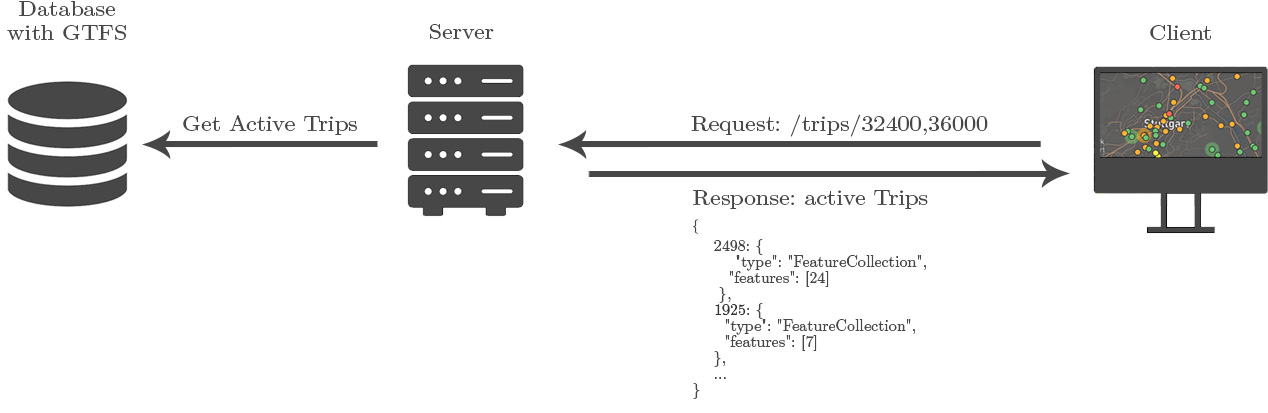
\includegraphics[width=\textwidth]{server_client.jpg}
      \caption{Server / Client Relation}
      \label{fig:server_client}
    \end{center}
  \end{figure}

  Trifft eine valide Anfrage auf den \texttt{/trips/:from,:to} Endpunkt, so wird ein Ablauf nach Abbildung \ref{fig:server_client} angestoßen.
  Die eintreffenden Anfragen werden vom Server entgegengenommen, validiert, verarbeitet und anschließend die entsprechende Antwort zurück gesendet. Die Validierung prüft die vom Client übergebenen Parameter auf ihre Plausibilität. Schlägt diese Prüfung fehl wird ein Fehler vom Server zurückgegeben und der Server wartet auf eine neue Anfrage. Die wichtigste Routine des Servers stellt die Abfrage von Trips aus der Datenbank dar. Die Datenbank sucht diejenigen Trips heraus, welche in dem benötigten Zeitraum \texttt{from, to} aktiv sind. Dabei wird das Datum und der Wochentag zum Zeitpunkt der Anfrage verwendet. Damit der Client bei der Animation möglichst wenig Rechenarbeit hat, werden alle Daten, bei denen dies möglichst ist, vorberechnet. Folgender Ablauf findet statt:

  \begin{itemize}
    \item \textbf{Daten Mapping:} Die Trips aus der Datenbank werden in das \texttt{GeoJSON}-Format umgewandelt, damit diese im weiteren Programmverlauf einfacher zu verarbeiten sind. Dabei werden die im Kapitel "`\ref{sub:begriffe} \nameref{sub:begriffe}"' festgelegten Definitionen beachtet.

    \item \textbf{Zurückgelegte Distanz:} Damit eine Animation der Vehicle stattfinden kann ist die Berechnung der Distanzen zwischen den einzelnen Stationen nötig. Falls das Feld \texttt{stops\_dist\_traveled}\footnotemark in der Datenbank vorhanden ist, kann die zurückgelegte Distanz sehr einfach daraus berechnet werden. Ist dies nicht der Fall so wird ein Station Matching durchgeführt, um die Distanzen berechnen zu können.
    \footnotetext{Die zurückgelegte Distanz bis zu einer Station $S$}

    \item \textbf{Station Matching:} Unter Station Matching versteht sich die Positionierung der Stationen auf und entlang der Polyline. Dies wird im nächsten Abschnitt ausführlicher betrachtet.

    \item \textbf{Feststellen der Richtung:} Für eine Polyline ist es unerheblich ob die Koordinaten in der Reihenfolge $\{ p_1, p_2, \dotsc, p_n \}$ oder $\{ p_n, \dotsc, p_2, p_1 \}$ angeordnet sind. Damit das Vehicle aber in die richtige Richtung von $A$ nach $B$ fährt, ist es wichtig dass die Koordinaten der Polyline in aufsteigender Reihenfolge festgelegt werden. Falls dies nicht er Fall ist, werden die Koordinaten in ihrer Reihenfolge umgekehrt.

    \item \textbf{Codieren der Polyline:} Zuletzt werden die Koordinaten in einen Polyline String Codiert und abschließend versendet.
  \end{itemize}

% subsubsection server (end)